\documentclass[tikz,border=5pt]{standalone}
\usepackage{xcolor}
\usepackage{tikz}
\usetikzlibrary{arrows.meta,positioning}
\usetikzlibrary{calc}

\begin{document}
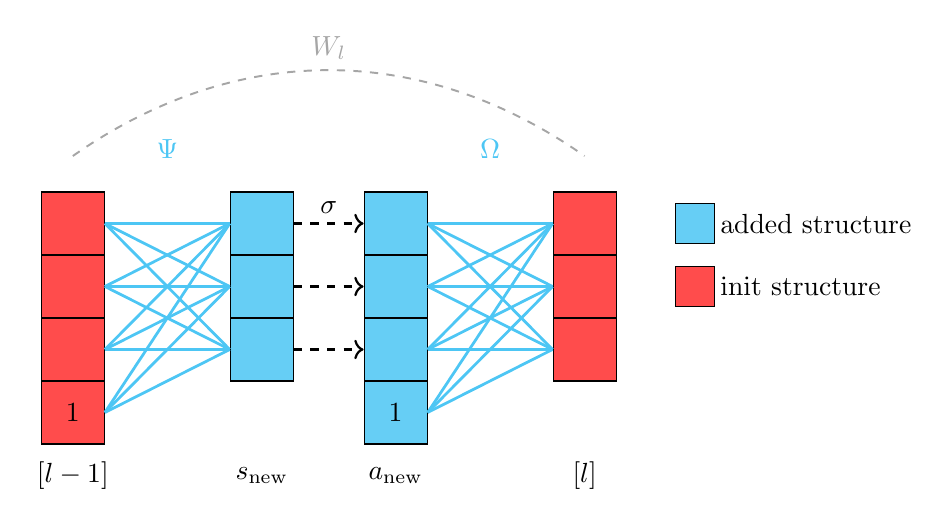
\begin{tikzpicture}[
    neuron/.style={draw, rectangle, minimum width=8mm, minimum height=8mm},
    redneuron/.style={neuron, fill=red!70},
    blueneuron/.style={neuron, fill=cyan!60},
    conn/.style={-, black!70, line width=0.6pt},
    oldconn/.style={-, black!35, dashed, line width=0.7pt},
    addconn/.style={-, cyan!70, line width=1pt},
    act/.style={->, dashed, line width=0.8pt}
]

% x positions of layers
\def\xA{0}
\def\xB{2.4}
\def\xC{4.1}
\def\xD{6.5}

% Existing left layer (h_{l-1}(x))
\foreach \i in {0,...,2} {
    \node[redneuron] (A\i) at (\xA, \i*0.8) {};
}
\node[redneuron] (Aone) at (\xA,-0.8) {1};
\node at (\xA,-1.6) {$\postact[l-1]$};

% Added preactivation layer (z_new)
\foreach \i in {0,...,2} {
    \node[blueneuron] (B\i) at (\xB, \i*0.8) {};
}
\node at (\xB,-1.6) {$s_{\rm new}$};

% Added postactivation layer (h_new)
\foreach \i in {0,...,2} {
    \node[blueneuron] (C\i) at (\xC, \i*0.8) {};
}
\node[blueneuron] (Cone) at (\xC,-0.8) {1};
\node at (\xC,-1.6) {$a_{\rm new}$};

% Existing right layer (z_l(x))
\foreach \i in {0,...,2} {
    \node[redneuron] (D\i) at (\xD, \i*0.8) {};
}
\node at (\xD,-1.6) {$\preact[l]$};

% Activation arrows
\draw[act] (B2) -- node[above] {$\sigma$} (C2);
\draw[act] (B1) -- (C1);
\draw[act] (B0) -- (C0);

% New dense connections h^{(l-1)} -> z_new
\foreach \i in {0,...,2} {
    \foreach \j in {0,...,2} {
        \draw[addconn] (A\i.east) -- (B\j.west);
    }
}
\foreach \j in {0,...,2} {
    \draw[addconn] (Aone.east) -- (B\j.west);
}

% New dense connections h_new -> z^{(l)}
\foreach \i in {0,...,2} {
    \foreach \j in {0,...,2} {
        \draw[addconn] (C\i.east) -- (D\j.west);
    }
}
\foreach \j in {0,...,2} {
    \draw[addconn] (Cone.east) -- (D\j.west);
}

% Original direct mapping, de-emphasized after insertion
\draw[oldconn] ($(A2.north)+(0,0.45)$) to[out=35,in=145] node[above] {$W_l$} ($(D2.north)+(0,0.45)$);

% Labels
\node[cyan!70] at (\xB-1.2,2.55) {$\Psi$};
\node[cyan!70] at (\xC+1.2,2.55) {$\Omega$};

% Legend (right side)
\node[blueneuron, minimum width=5mm, minimum height=5mm] at (7.9, 1.6) {};
\node[anchor=west] at (8.1, 1.6) {added structure};

\node[redneuron, minimum width=5mm, minimum height=5mm] at (7.9, 0.8) {};
\node[anchor=west] at (8.1, 0.8) {init structure};

\end{tikzpicture}
\end{document}
